\documentclass[border=3pt]{standalone}
\usepackage{tikz}
\begin{document}
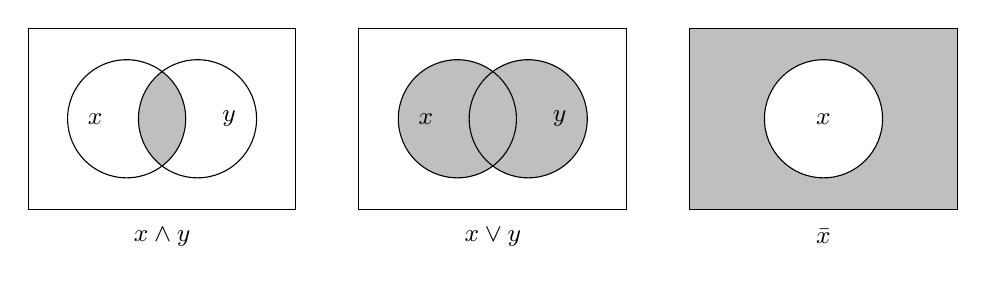
\begin{tikzpicture}[font=\sffamily\small]
  
  % AND: intersection
  \begin{scope}
    \begin{scope}
      \clip (-0.45,0) circle (0.75);
      \fill[black!25] (0.45,0) circle (0.75);
    \end{scope}
    \draw (-1.7,-1.15) rectangle (1.7,1.15);
    \draw (-0.45,0) circle (0.75) (0.45,0) circle (0.75);
    \node at (-0.85,0) {$x$};
    \node at (0.85,0) {$y$};
    \node at (0,-1.5) {$x \land y$};
  \end{scope}
  % OR: union
  \begin{scope}[xshift=4.2cm]
    \fill[black!25] (-0.45,0) circle (0.75);
    \fill[black!25] (0.45,0) circle (0.75);
    \draw (-1.7,-1.15) rectangle (1.7,1.15);
    \draw (-0.45,0) circle (0.75) (0.45,0) circle (0.75);
    \node at (-0.85,0) {$x$};
    \node at (0.85,0) {$y$};
    \node at (0,-1.5) {$x \lor y$};
  \end{scope}
  % NOT: outside
  \begin{scope}[xshift=8.4cm]
    \fill[even odd rule,black!25] (-1.7,-1.15) rectangle (1.7,1.15) (0,0) circle (0.75);
    \draw (-1.7,-1.15) rectangle (1.7,1.15);
    \draw (0,0) circle (0.75);
    \node at (0,0) {$x$};
    \node at (0,-1.5) {$\bar{x}$};
  \end{scope}
\end{tikzpicture}
\end{document}
